\documentclass{tecweb}

\title{Relazione progetto Tecnologie Web}

\begin{document}
	\begin{titlepage}
		\begin{center}
			
\includegraphics[width=5cm]{Logo2}
			\vspace{0.5cm}	\\
			\Huge \textbf{Serie-a-mente}
			\vspace{0.5cm}\\
			\normalsize \textbf{Progetto di Tecnologie Web}
			\vspace{0.7cm}	\\
			\renewcommand\arraystretch{1.3}	
			\begin{tabularx}{11cm}{r|X}
				\multicolumn{2}{c}{\textbf{Informazioni sul gruppo}}\\ 
				\hline
				\textbf{Componenti} & Marco Focchiatti \\ & Tommaso Loss \\ & Valentina Marcon \\  
				\textbf{Referente} & Valentina Marcon \\ 
				\textbf{Mail} & valentina.marcon3@studenti.unipd.it \\
			\end{tabularx}
			\vspace{0.7cm}
			\textbf{Indirizzo del sito:}
			\vspace{0.7cm}	\\
			\begin{tabularx}{11cm}{r|X}
				\multicolumn{2}{c}{\textbf{Dati Login}}\\ 
				\hline
				\textbf{Amministratore} & admin - admin \\
				\textbf{Utente} & user-user
			\end{tabularx}
		\vspace{2cm}
		\textit{Anno Accademico 2017-2018}
			
		\end{center}
	\end{titlepage}
	\tableofcontents
	\newpage
	\section{Abstract}
	Lo scopo del progetto è la realizzazione di un sito che svolga la duplice funzione di contenitore di informazioni, generali e particolari, riguardo alle serie televisive e di gestire un basilare sistema di votazione da parte degli utenti. In questo modo si facilita la scelta da parte di un utente riguardo a una nuova serie da seguire e si garantisce la possibilità di rimanere aggiornati rispetto alle serie seguite. \\
	L'interazione è prevista solamente fra le classi di utenza e il sito a causa dell'ampio e variegato target al quale si fa riferimento. L'utente infatti può aggiungere o rimuovere serie alla sua collezione virtuale, e votarle. L'amministratore gestisce le serie presenti nel sito, e le notizie riportate. \\
	Proprio a causa della varietà di utenza prevista è stato data priorità all'usabilità e all'accessibilità, utilizzando XHTML strict, in modo da garantire l'utilizzo del sito a prescindere dal contesto, rispettando lo standard del W3C.
	\newpage
	\section{Utenti Destinatari}
	Il sito si rivolge al pubblico, variegato come età e cultura, delle serie televisive. Sia come utenti veri e proprio che come utilizzatori occasionali interessati a informazione più o meno approfondite, riguardo l'argomento. Solo gli utenti iscritti possono votare le serie ma non è necessario il login per vedere l'indice di gradimento di una serie. Considerando che i destinatari sono molto eterogenei abbiamo deciso di non consentire interazione fra utenti, sotto forma di commenti alle serie, in quanto necessiterebbe di un notevole lavoro di moderazione.
	\newpage
	
	
	\section{Accessibilità} \label{Utenti destinatari}
	\subsection{Separazione fra comportamento, presentazione e struttura}
	Per mantenere al separazione fra comportamento, presentazione e struttura, fondamentale per l'accessibilità del sito, abbiamo sfruttato XHTML strict, php e CSS. In particolare, le pagine sono generate dinamicamente a partire da script php, che gestiscono la comunicazione con il database. I documenti XHTML strict fanno riferimento a fogli di stile esterni CSS per la presentazione.\\\
	Non dipendendo da Javascript, il sito rimane accessibile a un bacino di utenti molto elevato, allo stesso livello, rinunciando ad una grafica più accattivante, che per l'obiettivo che si pone il sito, è secondaria. \'E fondamentale invece allagare il più possibile il bacino di utenza.
	Infine abbiamo validato il codice in modo da avere la certezza di aderire agli standard W3C.
	\subsection{Tag per l'accessibilità}
	Ogni pagina è corredata dai relativi \textit{meta tag}, che descrivono gli elementi salienti del suo contenuto. \\
	Considerato l'elevato contenuto di termini inglesi è stato aggiunto l'attributo \textit{xml:lang="eng"}, dove necessario. \'E importante che l'ipotetico amministratore del sito corredi le aggiunte con gli adeguati tag linguistici, per preservare la corretta fruizione da parte di utenti utilizzanti screen-reader. Proprio per facilitare la lettura da parte di questi ultimi, si è fatto ricorso a immagini puramente accessorie, corredate da opportuni attributi alt descrittivi. \\
	Infine ogni form per l'input è descritto da una \textit{label} e inserito in un \textit{fieldset}.
	\subsection{Scelta dei colori}
	Abbiamo utilizzato colori semplici con un contrasto elevato, 
	%quale sito per verificare il contrasto?% 
	per permettere la fruizione a utenti con problemi alla vista. In più, colori seriosi si abbinano al carattere di utilità pratica del sito.
	Queste scelte sono state verificate tramite \textbf{Coblis}\footnote{\url{http://www.color-blindness.com/coblis-color-blindness-simulator/}}, un sito che permette di visualizzare la pagina come verrebbe vista da un utente con varie tipologie di daltonismo.\\
	\begin{minipage}{0.5\textwidth}
		\begin{figure}[H]
			\flushleft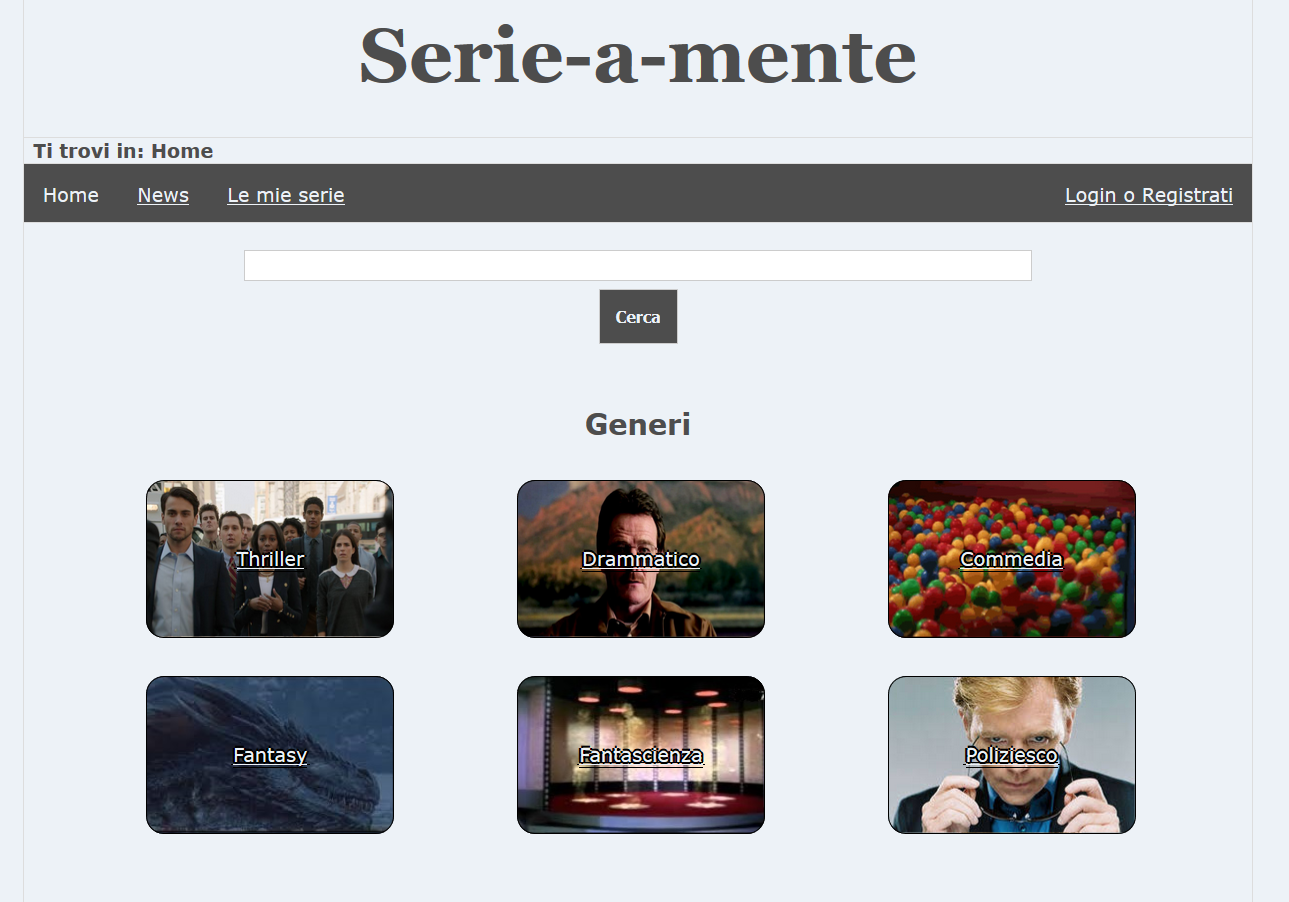
\includegraphics[width=7cm]{Home}
		\end{figure}
	\end{minipage}\hfill
	\begin{minipage}{0.5\textwidth}
		Fig 1: Pagina iniziale del sito	\\
	\end{minipage}
	\begin{minipage}{0.5\textwidth}
		\begin{figure}[H]
			\flushleft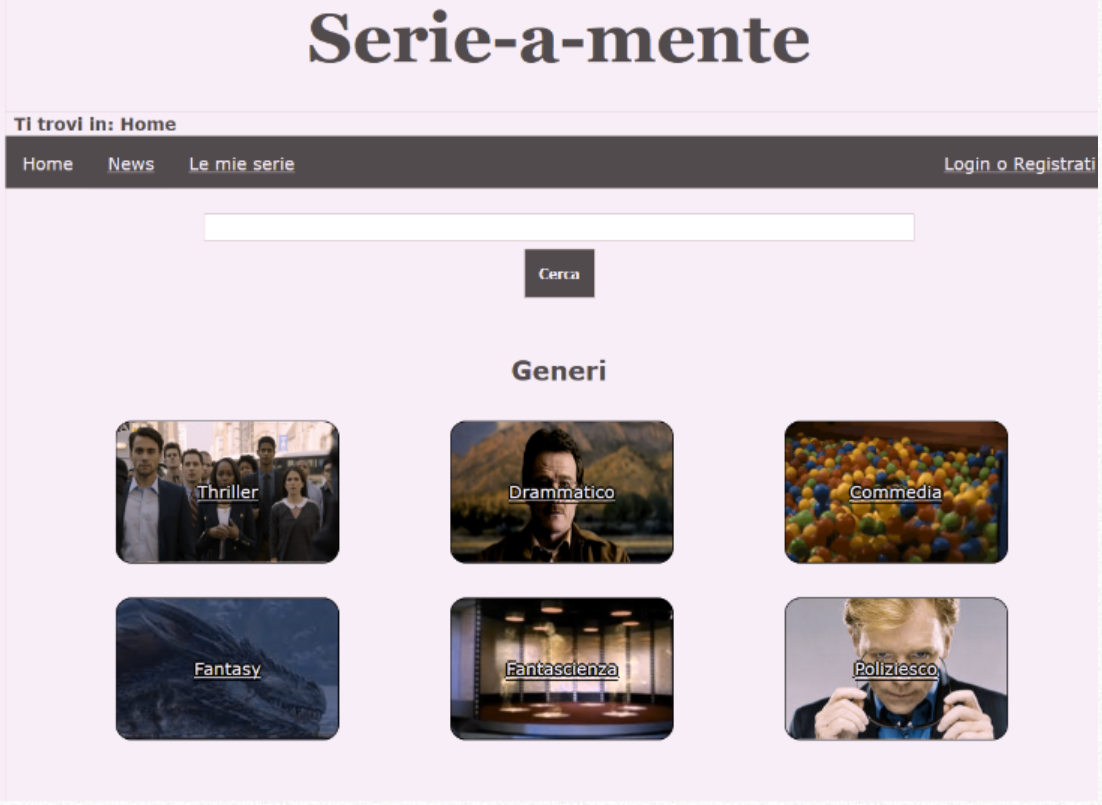
\includegraphics[width=7cm]{Deuteranope}
		\end{figure}
	\end{minipage} \hfill
	\begin{minipage}{1\textwidth}
		Fig 1: Home del sito vista da\\ un utente Deuteranope	\\
	\end{minipage}
	\begin{minipage}{0.5\textwidth}
		\begin{figure}[H]
			\flushleft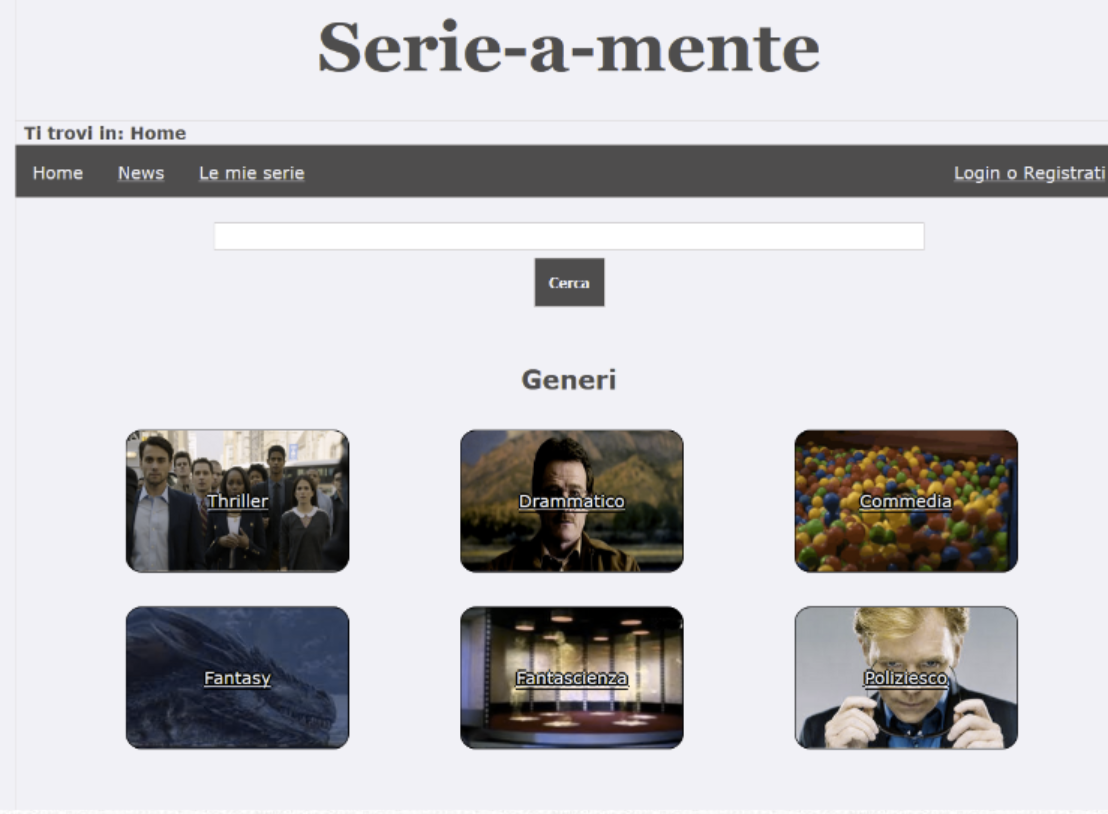
\includegraphics[width=7cm]{Protanope}
		\end{figure}
	\end{minipage} \hfill
	\begin{minipage}{1\textwidth}
		Fig 1: Home del sito vista da\\ un utente Protanope	\\
	\end{minipage}
	\begin{minipage}{0.5\textwidth}
		\begin{figure}[H]
			\flushleft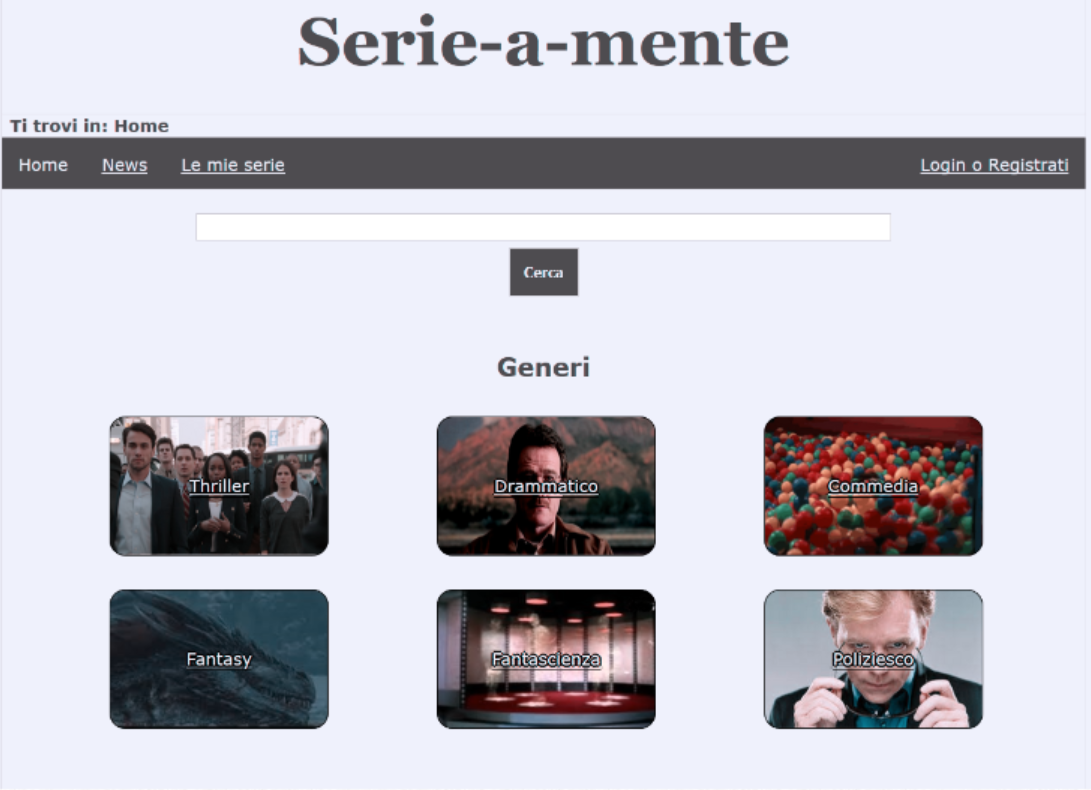
\includegraphics[width=7cm]{Tritanope}
		\end{figure}
	\end{minipage} \hfill
	\begin{minipage}{1\textwidth}
		Fig 1: Home del sito vista da\\ un utente Tritanope	\\
	\end{minipage}
	\vspace{0.5cm}
	
	I link sono evidenziati ovunque dalla sottolineatura e dal colore blu. Quelli già visitati, fatta eccezione per quelli nel menù, divengono grigi. 
	\subsection{Strumenti generici di accessibilità}
	Per ogni pagina sono forniti link per ritornare al menù, utili sia per gli utenti \textit{mobile} sia per la navigazione tramite screen-reader. Per questi ultimi è anche presente un link per saltare il menù e passare direttamente al contenuto, in modo da facilitare la navigazione.
	\newpage
	\section{Usabilità}
	
	\subsection{Navigabilità}
	Vengono forniti due strumenti per facilitare la navigazione:
	\begin{itemize}
		\item Breadcrumb: Viene sempre riportato il percorso effettuato dalla pagina iniziale del sito, per facilitare l'utente alla creazione di una mappa mentale.
		\item Menù: il menù è presente, sotto la breadcrumb, e riporta la pagina corrente senza la sottolineatura caratteristica dei link, in modo da evitare interazioni superflue. Le altre pagine vengono evidenziate quando sono sorvolate dal mouse, per chiarire la loro funzione. Si è scelto un menù orizzontale considerando il basso numero di voci richieste, meno invadente rispetto alla controparte verticale, riflettendo sul fatto che futuri ampliamenti del sito opereranno più probabilmente su funzionalità aggiuntive implementabili tramite bottoni o form e non su nuove voci del menù.
	\end{itemize}
	\subsection{Utilità attesa}
	Come analizzato nel paragrafo \ref{Utenti destinatari}, il sito fornisce il contenuto richiesto cioè informazioni di base riguardo a serie televisive, in modo da aiutare l'utente nella scelta e, opzionalmente, approfondimento tramite altre fonti.
	\subsection{Completezza dei contenuti}
	Questo parametro è dipendente dal lavoro dell'amministratore, se i contenuti sono coerenti, completi e mantenuti, la struttura del sito ne garantisce la giusta visualizzazione.
	\subsection{Comprensibilità delle informazioni}
	Tutta l'informazione è veicolata tramite testo in italiano, evitando immagini rappresentanti contenuto per ragioni di accessibilità. \'E quindi sufficiente una buona comprensione della lingua.
	\subsection{Efficacia comunicativa}
	Il sito è finalizzato completamente alla condivisione di informazioni, privilegiando l'approccio diretto, evitando qualsiasi orpello grafico aggiuntivo, i quale, seppur apprezzabili, potrebbero causare disorientamento o perdita del focus agli utenti.
	\subsection{Attrattività grafica}
	Per raggiungere gli obiettivi indicati precedentemente, abbiamo optato per un layout il più minimalista possibile.
	\newpage
	\section{Struttura}
	Per gestire l'iterazione con l'utenza, quasi tutte le pagine del sito sono dinamiche, in particolare, sono file \textit{php} che hanno come output un documento codificato in XHTML 1.0 Strict, per garantire una elevata retrocompatibilità. \\
	Qui di seguito, sono elencati tutti i documenti che producono file \path{html} e le loro funzioni:
	\subsection{Pagine raggiungibili da tutti gli utenti}
	\begin{itemize}
		\item \path{Home.php}: Pagina che rappresenta la Homepage del sito, mostra la barra di ricerca serie generica, e le 6 categorie nelle quali sono suddivise. %Abbiamo deciso di rendere non espandibile questa suddivisione, perché è raro ne si sviluppino di nuove.%
		Inoltre ciascuna serie ha una e una sola categoria principale, per evitare di confondere l'utente rispetto alla loro collocazione nel sito;
		\item \path{news.php}: Pagina che raccoglie le notizie riguardo alle serie presenti nel sito, viene aggiornata dall'amministratore a sua discrezione;
		\item \path{Drammatico/Fantasy/Poliziesco/Thriller/Commedia/Fantascienza.php}: Pagine che contengono la lista delle serie appartenenti al genere in questione, con riferimento alla pagina specifica della serie, e la loro valutazione media;
		\item \path{Ricerca.php}: Pagina che mostra tutte le serie che corrispondono alla query inserita, completamente o parzialmente, insieme a genere e valutazione media;
		\item \path{Serie.php}: Pagina che raccoglie le informazioni generali della serie ricercata o indirizzata;
		\item \path{Login.php}: Pagina che permette l'accesso a un utente iscritto, tramite la scrittura del nome utente e della password corretti;
		\item \path{Registrazione.php}: Pagina che permette la registrazione di un nuovo utente, tramite la scelta di un nickname e di una password;
		\item \path{RegistrazioneEffettuata.%php.html???%
		}: Pagina che conferma la registrazione all'utente che ha effettuato correttamente la procedura.
	\end{itemize}
	\subsection{Pagine raggiungibili dagli utenti registrati}
	\begin{itemize}
		\item \path{Serie.php}: Pagina che raccoglie le informazioni generali della serie ricercata o indirizzata, un utente registrato può anche aggiungere la serie alla sua collezione personale, se mancante, oppure rimuoverla, se presente;
		\item \path{Mypage.php}: Pagina che visualizza le serie scelta dall'utente e permette di valutarle o modificarne la valutazione.
	\end{itemize}
	\subsection{Pagine raggiungibili dagli amministratori}
	\begin{itemize}
		\item \path{Addserie.php}: Pagina che permette all'amministratore di aggiungere una serie a quelle presenti nel database;
		\item \path{Addnews.php}: Pagina che permette all'amministratore di aggiungere una notizia a quelle presenti nel database;
		\item \path{Modserie.php}: Pagina che permette all'amministratore di modificare i dati di una serie, viene acceduta dalla specifica pagina della serie tramite un link.
	\end{itemize}
	\newpage
	\section{Presentazione}
	Per quanto riguarda la presentazione abbiamo sfruttato fogli di stile seguendo lo standard CSS3. Gli unici elementi critici per quanto riguarda la compatibilità, cioè immagini e bordi arrotondati, sono puramente accessori. Le immagini della Home, di puro abbellimento, sono gestite come background e quindi ignorate da eventuali screen-reader.\\
	I file \path{css} sono i seguenti:
	\begin{itemize}
		\item \path{styledesktop.css}: Foglio di stile che si occupa del layout del sito per utente desktop;
		\item \path{stylephone.css}: Foglio di stile che gestisce il layout per utente mobile;
		\item \path{stylesmall.css}: Foglio di stile che provvede al ridimensionamento fluido dell'interfaccia quando si riducono le dimensioni della finestra;
		\item \path{styleprint.css}: Foglio di stile che adatta il sito alla stampa.		
	\end{itemize}
	\newpage
	\section{Comportamento}
	Il comportamento del sito, il quale riguarda principalmente l'interazione fra utenti e il database, è sviluppato tramite script php. Abbiamo deciso di non utilizzare Javascript per non distogliere l'attenzione dell'utente occasionale, per ridurre al minimo la durata delle sessioni richieste e per evitare quando possibile problemi di compatibilità.\\
	Sono presenti due file che non producono direttamente una pagina \path{html}, bensì contengono delle funzioni di uso comune che vengono richiamate negli altri file:
	\begin{itemize}
		\item \path{DBAccess.php}: In questo file sono presenti le funzioni per dialogare con il database, cioè per gestire la connessione e svolgere le varie query richieste dal sito;
		\item \path{DataWriter.php}: Questo file racchiude le funzioni generiche e di base per stampare i dati ottenuti da \path{DBAccess.php}.
	\end{itemize}
	La maggior parte dei file rimanenti, già trattati precedentemente, contiene elementi in php necessari per la generazione delle pagine \path{html} dinamiche.
	\newpage
	\section{Gestione dei dati}
	I dati utili al sito sono memorizzati in un database relazionale, \path{DB.sql}. Esso contiene 4 tabelle:
	\begin{itemize}
		\item SerieTv: contenente i dati relativi alle serie televisive memorizzate (titolo, genere, data d'inizio, data di fine, numero stagioni e trama);
		\item Notizie: contenente i dati relativi alle notizie  memorizzate (titolo, genere, data d'inizio, data di fine, numero stagioni e trama);
		\item Utente: contenente i dati relativi agli utenti (nickname, password e se è amministratore);
		\item Valutazione: contenente le valutazioni degli utenti (titolo della serie, voto e nickname dell'utente).
	\end{itemize}
	In più sono presenti una \textit{view} e tre \textit{trigger}, per gestire gli aggiornamenti delle dei voti e la media di ciascuna serie.
	
	\newpage
	\section{Validazione e Test}
	\'E stata effettuata una necessaria opera di validazione per confermare la corretta fruizione del sito da parte delle più variegate possibili tipologie di browser, in modo da confermare l'obiettivo iniziale.
	\subsection{Validazione}
	La validazione è stata verificata tramite i servizi forniti dal W3C, sia per i documenti \path{html} sia per quelli \path{css}, per i primi tramite
	 il CSS validation service \footnote{\url{https://jigsaw.w3.org/css-validator/}} e per i secondi utilizzando il Markup validation service\footnote{\url{http://validator.w3.org/}}.
	\subsection{Test}
	I test sono stati effettuati su una macchina con Windows 10, eccetto che per safari che è stato testato su un sistema operativo macOS Sierra. Per le varie versioni di Internet Explorer antecedenti all'11 abbiamo utilizzato gli strumenti per sviluppatori di IE 11 i quali, sebbene non siano accuratissimi, danno una buona approssimazione del risultato atteso.
	\begin{itemize}
		\item \textbf{Chrome 64}: sito correttamente visualizzato;
		\item \textbf{Safari 11}: sito correttamente visualizzato;
		\item \textbf{Firefox 58}: sito correttamente visualizzato;
		\item \textbf{Opera 50}: sito correttamente visualizzato;
		\item \textbf{Edge 41}: sito quasi completamente supportato;
			\begin{itemize}
				\item la sottolineatura dei generi nella home compre leggermente il testo.
			\end{itemize}
	 	\item \textbf{IE 11}: sito quasi completamente supportato;
	 		\begin{itemize}
	 			\item la sottolineatura dei generi nella home compre leggermente il testo.
	 		\end{itemize}
	 	\item \textbf{IE 10}: sito quasi completamente supportato;
	 		\begin{itemize}
	 			\item la sottolineatura dei generi nella home compre leggermente il testo.
	 		\end{itemize}
	 	\item \textbf{IE 9}: sito quasi completamente supportato;
	 		\begin{itemize}
	 			\item non vengono visualizzati i bordi ai generi nella home rendendoli meno leggibili.
	 		\end{itemize}
		%\item \textbf{IE 8/7/6}:
		%	\begin{itemize}
		%		\item 
		%		\item 
		%		\item 
		%		\item 
		%	\end{itemize}
	\end{itemize}
	\newpage
	\appendix
	\section{Organizzazione del gruppo}
	Ogni mebro ha svolto determinati compiti, qui riportati:
	\begin{itemize}
		\item \textbf{Marco Focchiatti}:
		\begin{itemize}
			\item Creazione della struttura in PHP;
			\item Lavoro sulla parte generale di struttura;
			\item Modifiche alla presentazione;
			\item Lavoro sul database;
		\end{itemize}
		\item \textbf{Tommaso Loss}:
		\begin{itemize}
			\item Creazione e popolamento del database;
			\item Aggiunta funzioni amministratore;
			\item Aggiunta funzioni di accessibilità del sito;
			\item Stesura della relazione;
		\end{itemize}
		\item \textbf{Valentina Marcon}:
		\begin{itemize}
			\item Creazione dei file css;
			\item Scrittura della parte di presentazione del sito;
			\item Aggiunta funzioni di accessibilità del sito;
			\item Aggiunta funzioni utente registrato.
		\end{itemize}
	\end{itemize}
\end{document}